% One-page layout: (proof-)reading on display
%%%% \documentclass[11pt,oneside,a4paper]{book}
% Two-page layout: final printing
\documentclass[11pt,twoside,a4paper]{book}   
%=-=-=-=-=-=-=-=-=-=-=-=--=%
% The user of this template may find useful to have an alternative to these 
% officially suggested packages:
\usepackage[czech, english]{babel}
\usepackage[T1]{fontenc} % pouzije EC fonty 
% pripadne pisete-li cesky, pak lze zkusit take:
% \usepackage[OT1]{fontenc} 
\usepackage[utf8]{inputenc}
%=-=-=-=-=-=-=-=-=-=-=-=--=%
% In case of problems with PDF fonts, one may try to uncomment this line:
%\usepackage{lmodern}
%=-=-=-=-=-=-=-=-=-=-=-=--=%
%=-=-=-=-=-=-=-=-=-=-=-=--=%
% Depending on your particular TeX distribution and version of conversion tools 
% (dvips/dvipdf/ps2pdf), some (advanced | desperate) users may prefer to use 
% different settings.
% Please uncomment the following style and use your CSLaTeX (cslatex/pdfcslatex) 
% to process your work. Note however, this file is in UTF-8 and a conversion to 
% your native encoding may be required. Some settings below depend on babel 
% macros and should also be modified. See \selectlanguage \iflanguage.
%\usepackage{czech}  %%%%%\usepackage[T1]{czech} %%%%[IL2] [T1] [OT1]
%=-=-=-=-=-=-=-=-=-=-=-=--=%

%%%%%%%%%%%%%%%%%%%%%%%%%%%%%%%%%%%%%%%
% Styles required in your work follow %
%%%%%%%%%%%%%%%%%%%%%%%%%%%%%%%%%%%%%%%
\usepackage{graphicx}
%\usepackage{indentfirst} %1. odstavec jako v cestine.
\usepackage{setspace}
\usepackage[hyphens]{url}
\usepackage{pgfplots}

\usepackage{misc/k336_thesis_macros} % specialni makra pro formatovani DP a BP
 % muzete si vytvorit i sva vlastni v souboru k336_thesis_macros.sty
 % najdete  radu jednoduchych definic, ktere zde ani nejsou pouzity
 % napriklad: 
 % \newcommand{\bfig}{\begin{figure}\begin{center}}
 % \newcommand{\efig}{\end{center}\end{figure}}
 % umoznuje pouzit prikaz \bfig namisto \begin{figure}\begin{center} atd.

\newcommand\TypeOfWork{Master's Thesis}   \typeout{Master's Thesis} 
\newcommand\StudProgram{Open Informatics}
\newcommand\StudBranch{Software Engineering}

%%%%%%%%%%%%%%%%%%%%%%%%%%%%%%%%%%%%%%%%%%%%
% Vyplnte nazev prace, autora a vedouciho
% Set up Work Title, Author and Supervisor
%%%%%%%%%%%%%%%%%%%%%%%%%%%%%%%%%%%%%%%%%%%%

\newcommand\WorkTitle{Semantic Data Analysis and Visualization of User Interactions}
\newcommand\FirstandFamilyName{Bc. Michal Švácha}
\newcommand\Supervisor{Ing. Ivo Malý Ph.D.}


% Pouzijete-li pdflatex, tak je prijemne, kdyz bude mit vase prace
% funkcni odkazy i v pdf formatu
\usepackage[
pdftitle={\WorkTitle},
pdfauthor={\FirstandFamilyName},
bookmarks=true,
colorlinks=true,
breaklinks=true,
urlcolor=red,
citecolor=blue,
linkcolor=blue,
unicode=true,
]
{hyperref}

\usepackage{listings}
\usepackage{color}

\definecolor{dkgreen}{rgb}{0,0.6,0}
\definecolor{gray}{rgb}{0.5,0.5,0.5}
\definecolor{mauve}{rgb}{0.58,0,0.82}

\lstset{frame=tb,
  language=Java,
  aboveskip=3mm,
  belowskip=3mm,
  showstringspaces=false,
  columns=flexible,
  basicstyle={\small\ttfamily},
  numbers=none,
  numberstyle=\tiny\color{gray},
  keywordstyle=\color{blue},
  commentstyle=\color{dkgreen},
  stringstyle=\color{mauve},
  breaklines=true,
  breakatwhitespace=true,
  tabsize=3
}

\begin{document}

%%%%%%%%%%%%%%%%%%%%%%%%%%%%%%%%%%%%%
% Zvolte jednu z moznosti 
% Choose one of the following options
%%%%%%%%%%%%%%%%%%%%%%%%%%%%%%%%%%%%%
%\selectlanguage{czech}
\selectlanguage{english} 

% prikaz \typeout vypise vyse uvedena nastaveni v prikazovem okne
% pro pohodlne ladeni prace


\iflanguage{czech}{
	 \typeout{************************************************}
	 \typeout{Zvoleny jazyk: cestina}
	 \typeout{Typ prace: \TypeOfWork}
	 \typeout{Studijni program: \StudProgram}
	 \typeout{Obor: \StudBranch}
	 \typeout{Jmeno: \FirstandFamilyName}
	 \typeout{Nazev prace: \WorkTitle}
	 \typeout{Vedouci prace: \Supervisor}
	 \typeout{***************************************************}
	 \newcommand\Department{Katedra počítačů}
	 \newcommand\Faculty{Fakulta elektrotechnická}
	 \newcommand\University{České vysoké učení technické v Praze}
	 \newcommand\labelSupervisor{Vedoucí práce}
	 \newcommand\labelStudProgram{Studijní program}
	 \newcommand\labelStudBranch{Obor}
}{
	 \typeout{************************************************}
	 \typeout{Language: english}
	 \typeout{Type of Work: \TypeOfWork}
	 \typeout{Study Program: \StudProgram}
	 \typeout{Study Branch: \StudBranch}
	 \typeout{Author: \FirstandFamilyName}
	 \typeout{Title: \WorkTitle}
	 \typeout{Supervisor: \Supervisor}
	 \typeout{***************************************************}
	 \newcommand\Department{Department of Computer Science and Engineering}
	 \newcommand\Faculty{Faculty of Electrical Engineering}
	 \newcommand\University{Czech Technical University in Prague}
	 \newcommand\labelSupervisor{Supervisor}
	 \newcommand\labelStudProgram{Study Programme} 
	 \newcommand\labelStudBranch{Field of Study}
}


%%%%%%%%%%%%%%%%%%%%%%%%%%    Titulni stranka / Title page 

\coverpagestarts

%%%%%%%%%%%%%%%%%%%%%%%%%%%    Podekovani / Acknowledgements 

\acknowledgements
\noindent
I would like to thank dearly to my cat, dog and goldfish I never had. You were a true inspiration to me. With you, I would have never made this document happen. Also, my PlayStation 3 proved to be an amazing tool to keep me sane while writing this thesis. Thank you SONY.


%%%%%%%%%%%%%%%%%%%%%%%%%%%   Prohlaseni / Declaration 

\declaration{In Prague on May 27, 2016}


%%%%%%%%%%%%%%%%%%%%%%%%%%%%    Abstract 
 
\abstractpage

The current status quo in data collection is to collect everything that is available. This approach has given rise to a trend in the last couple years - "Big Data". Data that is inconveniently large for processing, interpretation and inference. When a company decides to leverage big data, it usually ends up having too much information and no real business value. Each department uses different domain vocabularies and there is therefore no synchronization or understanding. This master's thesis is trying to take the opportunity of this disorder and connect the endpoints together while leveraging big data to provide an end-to-end solution.

The focal part of this thesis is the focus on user interactions - the collection of data from mobile applications. Before such collection can even happen, the interactions must be defined - the "what", "when" and "why". Starting with management, over to architecture and engineering to interpreting results as the destination - uniting all steps to form a bigger picture.


\vglue40mm

\noindent{\Huge \textbf{Abstrakt}}
\vskip 2.1\baselineskip

\noindent
Momentální status quo ve sběru dat je sbírání a ukládání všeho, co je k dispozici. Tento přístup dal vzniknout trendu posledních let - "Velká data". Tedy data, která jsou  nepohodlně objemná pro zpracování, výklad, a odvozování závěrů. Když se společnost rozhodne, že chce využít velká data, dopadne to většinou tak, že má příliš mnoho informací bez žádné reálné hodnoty. Každé oddělení používá vlastní doménové názvosloví a tudíž chybí synchronizace a porozumění. Tato diplomová práce se snaží využít této příležitosti neuspořádanosti pro spojení všech konců dohromady a vytvořit tak komplexní řešení.

Těžištěm práce je zaměření se na uživatelské interakce - sběr dat z mobilních aplikací. Než nějaký sběr vůbec nastane, je třeba mít interakce definované - tedy "co", "kdy" a "proč". Počínaje projektovým managementem, přes architekturu a softwarové inženýrství až k interpretaci výsledků jako konečným bodem - spojení všech kroků k vytvoření uceleného náhledu.


%%%%%%%%%%%%%%%%%%%%%%%%%%%%%%%%  Obsah / Table of Contents 

\tableofcontents


%%%%%%%%%%%%%%%%%%%%%%%%%%%%%%%  Seznam obrazku / List of Figures 

\listoffigures


%%%%%%%%%%%%%%%%%%%%%%%%%%%%%%%  Seznam tabulek / List of Tables

\listoftables


%**************************************************************

\mainbodystarts
% horizontalní mezera mezi dvema odstavci
%\parskip=5pt
\normalfont
\parskip=0.2\baselineskip plus 0.2\baselineskip minus 0.1\baselineskip

% Odsazeni prvniho radku odstavce resi class book (neaplikuje se na prvni 
% odstavce kapitol, sekci, podsekci atd.) Viz usepackage{indentfirst}.
% Chcete-li selektivne zamezit odsazeni 1. radku nektereho odstavce,
% pouzijte prikaz \noindent.
% \textit{práci implementační}, viz \cite{infodp} respektive \cite{infobp}.

%*****************************************************************************

\chapter{Introduction}

In lean/agile product development, it is necessary to have formalized user feedback loops in place, to measure product performance against various (quantitative) metrics. Such feedback loops obtain the information and statistics regarding user engagement and interaction with the developed product. Are the users using it the way the creator imagined or did they find any other means of utilizing it? What stops the users from doing the task they intended to do? Do they get everything they need, and at the same time, does the creator get what was expected? In other words, are the dominant means of usage incentive compatible for the users? 

Not only do the current solutions for gathering such user data for both quantitative and qualitative metrics work out-of-the-box with low-level semantics only (everything is a general activity on a general resource), but they also tend to run on somebody else's servers. What if the product developer is in a highly regulated market, such as pharmaceuticals, and has to own all their users' data? How can the current solutions' space be utilized and tweaked in order to fit such a schema?

\subsection*{Data Disconnectivity}

The most problematic issue in large corporations is the semantic disconnectivity of the data. This occurs when data is collected ad hoc without any set direction or goal to be achieved. It may physically be all there, however nobody knows what or how it should be connected in order for it to make sense and drive value. Do I have good data or do I just have petabytes of useless log trace? Am I gathering information on what the application was intended to do or am I only filling the database with irrelevant garbage information. Most importantly though, am I gathering the information I need in a consistent fashion that corresponds to the domain of the shareholders?

Let's draw an analogy here and let me illustrate the problem with a real-world example.

\newpage

\subsection*{Example}

\begin{figure}[!ht]
	\centering
	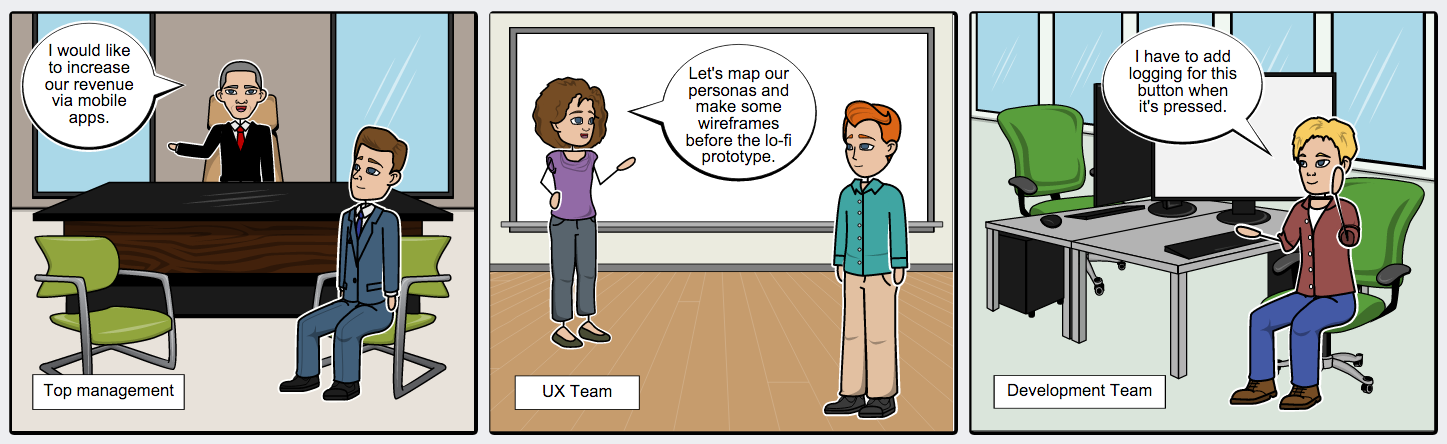
\includegraphics[width=0.9\textwidth]{figures/storyboard}
    \caption{Real-World Example}
\end{figure}

This situation is mainly caused by:

\begin{enumerate}
	\item Top management comes with a need to increase revenue via mobile devices.
	\item Project management team takes over and breaks it down to user-stories, tasks etc.
	\item Project management team asks the UX team, the mobile applications team and the backend team to perform their tasks in order to bring the product to life.
	\item By the time product development is spread across three different teams, it is very much likely that each team will create their own jargon for every activity performed in the product.
		\begin{itemize}
			\item The UX team is driven by the larger picture so they tend to refer to objects in a highly abstract way.
			\item The backend team is driven by the inner processes happening between the database and the REST API, so they speak their precise technical language.
			\item The mobile applications team is somewhere in-between, but never really aligned with either of the other teams.
		\end{itemize}
	\item When the product is delivered, the project management team has a really hard time translating the reported results into the top management's primary goals. Plus, the larger the teams are, the worse the situation actually gets.
\end{enumerate}

This isn't a problem of poor project management. The company can use the best project management tools on the market and have the smartest people working on their teams and still encounter this problem on a daily basis. This is a larger problem resulting from the lack of intersection between different domains (Management, UX, Development, DevOps).

\newpage

\section{Work Environment}

The context of this work is a large company, operating in a regulated market, where products are developed across multiple departments varying not only in size and experience, but also in project management approach - traditional and agile methods. Both methods implemented in the organization have a common denominator: measured KPIs to report the status of the work.

\subsection{Key Performance Indicators}

Each department/team/person has very specific Key Performance Indicators (= KPIs) that represent the value of their work. Even products have their KPIs - "How much value has this product brought?", "How much time is this product saving us?", etc.

\subsection{Software Development Life Cycle}

Software Development Life Cycle (= SDLC) is a standardized traditional and formalized approach to developing a software product for regulated markets. It enables companies to follow specific steps in order to get their software product certified for use in constrained environments. It is used not for the sake of bureaucracy, but to protect the customers and increase the level of traceability of a problem, should one ever occur.

\subsection{Agile Development Methodologies}

In the modern era of software development, it has become "cool" to not follow traditional waterfall models and to adopt agile methodologies, such as scrum or kanban. For many years these were found exclusively in start-ups. But because time and time again, research \cite{947100} has shown that agile methodologies do impact the level of productivity and innovation, larger companies are working on adopting them in their constrained context as well. This thesis operates in such a place, where agile methodologies are being deployed across the whole innovation department.

\section{Personal Interviews}

In order to find out what needs there are, I have conducted several interviews with leaders of various departments. These are their reactions to what bothers them about product monitoring during the development phase:

\begin{enumerate}
		\item Associate Director, Applied Technology
		\begin{itemize}
				\item[] "The real problem I see is the fact that all the information I need is on somebody else's server. We can't store any sensitive, let alone confidential information \emph{somewhere} with some random vendor. It's actually illegal in some countries. Unfortunately, sometimes sensitive data is exactly what we need to obtain from the applications to make an informed decision."
		\end{itemize}	

		\item Associate Director, Mobile and Web
		\begin{itemize}
				\item[] "Our needs for tracking KPIs are variable throughout time and unfortunately the current tools we use are quite inflexible. Because we are in a regulated market, each change that requires a new build of an application takes a longer period of time. And time \emph{is} money."
		\end{itemize}				
		
		\item Mobile Application Development Lead
		\begin{itemize}
				\item[] "I have noticed that one of the biggest obstacles is how should we name what we measure. I have no vocabulary to help me during the development. The only thing we have is a robust Google Analytics toolkit that only allows us to gather low-level actions. We can log that a button was pressed, but what do we name such action? "Button pressed"?"
		\end{itemize}
		
		\item UX Lead
		\begin{itemize}
				\item[] "Our team looks at the high-level needs. We are trying to make the user activities in an application as smooth as possible. When we design a low-fidelity prototype, we know what we want to measure. Having the opportunity to add a high-level KPI would help us a lot in order to gather feedback for our prototypes. We are not programmers, we don't know how to add it to the code, but I would love the idea of including what to measure along with the prototype."
		\end{itemize}
\end{enumerate}

\section{Scope of Work}

First, I will present the context of agile software development in a regulated market. Then I will take a look at the current tracking solutions being used in mobile development (the focus is on iOS development, but most of the tools are multiplatform solutions). I will examine and analyze their strengths and weaknesses. 

Next I will propose a workflow to fit the needs of a larger company with multiple departments, operating in a regulated market. I will utilize existing tools and build on top of them in order to drive value without reinventing the wheel couple times.

Lastly, I will develop a working PoC (Proof of Concept), verify its functions through user testing and further discuss with the stakeholders whether or not it is the correct path to take in order to unite all departments and connect the dots in the data.

\chapter{Analysis}

\section{Product Opportunity Assessment}

Product opportunity assessment is a helpful procedure to separate the wheat from the chaff. It points out the real pressing issues that are mission critical for the company.

\begin{enumerate}
	\item \emph{What problem are we trying to solve?}
	\item[] Enabling alignment of business language and user interaction reporting is a key part to a success of a new product. No commercially successful platforms allow such alignment, not even any higher semantic analysis. 
	\item[] In a regulatory market it is vital to have an option of storing the user data on custom servers. No such option along with the higher-level analysis is currently available at the market.
	\item[] There is no standardized toolkit and thus the lack of interchangeability between tools tends to end up with a vendor lock-in.
	
	\item \emph{For whom do we solve that problem?}
	\item[] 	For all departments in the company that are participating in product development, top to bottom. From setting a business goal to defining the needs, while also helping the developers and the designers.
	
	\item \emph{How will we measure success?}
	\item[] Having gathered data that is securely placed on custom servers. Data that is united and connected by shared domain vocabulary, ready to be analyzed and visualized in order to draw conclusions.

	\item \emph{What alternatives are out there?}
	\item[] There is some proprietary software on the market, but none is flexible enough for the defined needs.

	\item \emph{Why now?}
	\item[] The competitors \cite{data-driven-pharma} are really getting into the data-driven decisions. The intention is not to gather as much data as possible, but to generate valuable insights as soon as possible in order not to fall behind the competition.

	\item \emph{What factors are critical to success?	}
	\item[] Alignment of all departments participating in software development in a non-invasive fashion. It is critical to primarily focus on helping the departments to connect with each other.
	\item[] The ability to run the whole solution on custom servers and have total control over all gathered data.
	
\end{enumerate}


\section{Regulated environment constraints}

Regulated markets, especially pharmaceuticals have multiple rules that need to be carefully followed in order to be allowed to use their new IT products. Not only is important how much value does the final product bring to the end-user, but also how data storage is handled and how prone it is to exploitations and attacks. 

From the development process point of view it is equally important to follow specific guidelines and processes during the development phase. Each step has to be carefully documented and approved by specific audit department. For that reason, most of the big pharmaceutical companies use the waterfall model implemented in SDLC. It enables companies to follow these specific steps in order to get their software product certified. This all hassle is not for the sake of bureaucracy, it is to protect the customers and increases the level of tracability of a problem, should one ever occur. After all, it is theirs and their customers' private data that goes on the server, so it is imperative that it is safe.

The limitation of this approach is the inflexibility of the waterfall model. The strict and rigorous requirements for the waterfall model are not allowing to go back half way through and re-define the objectives of a product. Therefore more and more large companies are trying to implement the best of both worlds \cite{agile-waterfall}.

\begin{figure}[!ht]
	\centering
	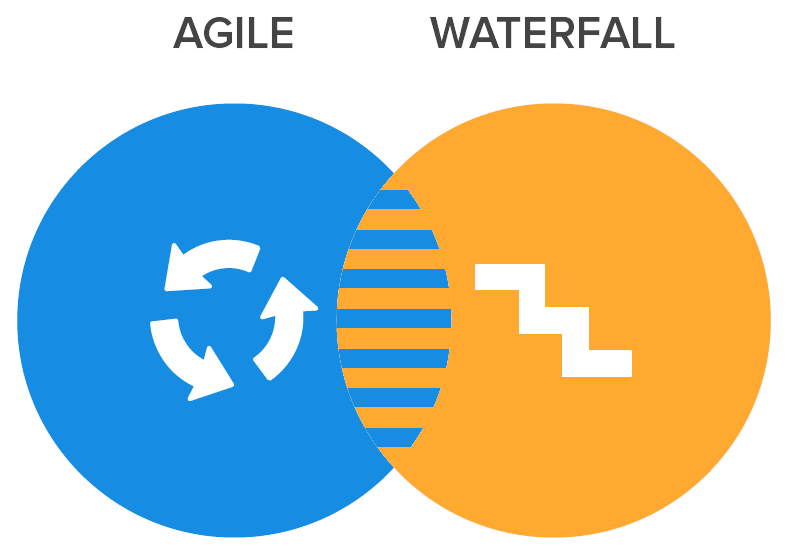
\includegraphics[width=0.4\textwidth]{figures/agile-waterfall}
    \caption{Balanced Approach to Waterfall and Agile Methodologies}
\end{figure}

In the context of my work, the approach is that prototypes, PoCs and internal beta versions of new software products are developed using various Agile Methodologies (Scrum and Kanban) and once their purpose is verified, the work done is considered as the starting point for the SDLC.

\section{Current Workflow}

Currently, the top management is in the USA, while the innovation department is in Prague, Czech Republic. Some members from the top management occasionally fly to Prague, but very irregularly and mostly for a quick check on the overall status of the department. Most of the communication happens remotely - via video conference calls, e-mails etc. Obviously, this produces a lot of noise in the data being transferred. Sometimes some parts are misheard or misunderstood, get lost and are causes for a larger problem in the future.

Not only there is a difference in the culture and language, but it clearly leads to a difference in the domain vocabularies used in everyday work. Tools for productive data exchange are implemented - such as:

\begin{itemize}
	\item Issue tracker
	\item Internal Wiki-style website
	\item Enterprise chat
\end{itemize}

But the problem is, that there is no tool that unites them all to make sure that the domain vocabularies are the same throughout the whole development phase. If such tool existed, a one that could connect to all of the deployed knowledge systems, it would make communication of measured performance of a product a lot easier.

Let's take a look at the current tools available on the market that specialize in application performance measuring.

\section{Existing Tools}

I will now analyze and assess the tools available on the market. I'll focus primarily on the flexibility of the deployment and their analysis features. Anything else has a minor priority.

\subsection{Google Analytics}

Google Analytics is by far the most popular and widely used framework for monitoring user interactions in applications. It reports everything the developer wishes to. By default it does not report anything - the tool has to be activated during application start. Then each action needs to be hard-coded in the code. An action can be two things - the first one is after a certain user activity has happened - a press of a button, pulling down a list to refresh the data etc. One thing gets reported - "this event has happened". The second one is more open - an identifier is set to an item, let's say, a button. Whatever happens with that button gets reported, be it touch, swipe or anything else.

\begin{figure}[!ht]
	\centering
	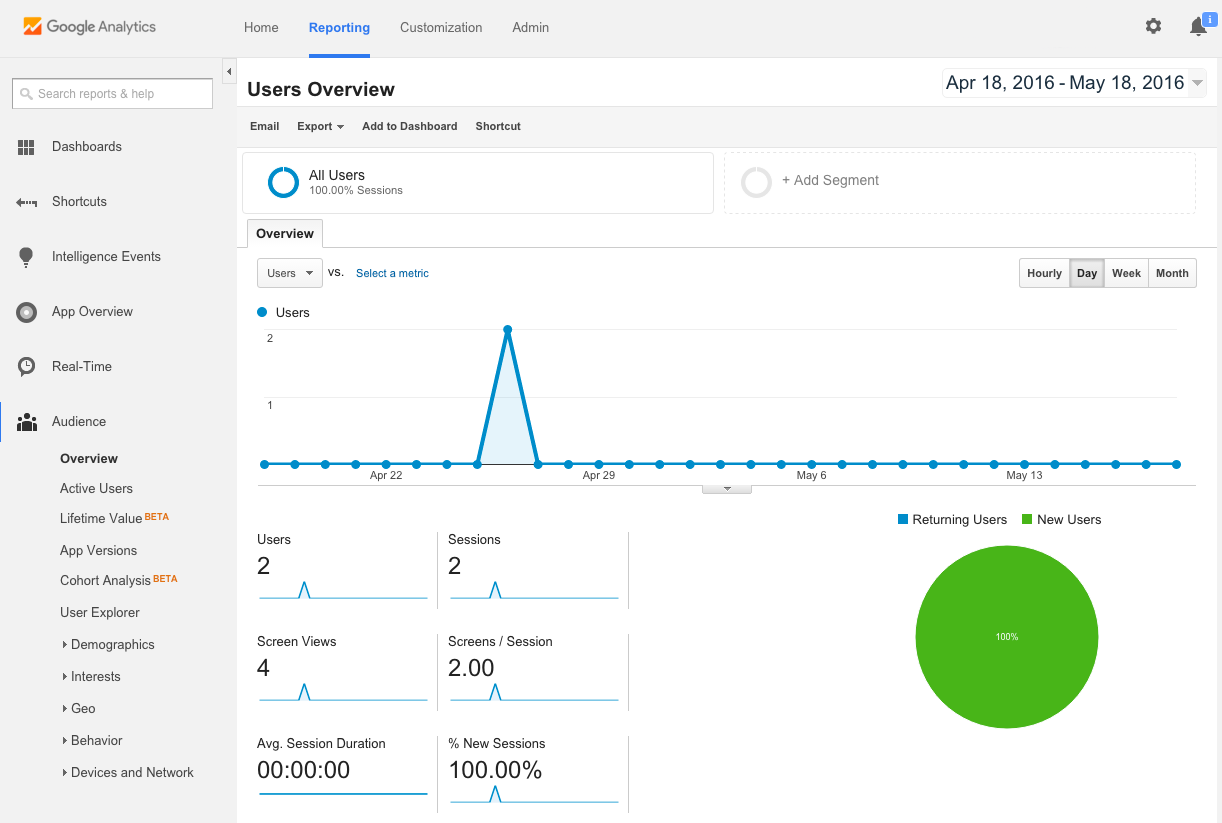
\includegraphics[width=0.65\textwidth]{figures/analytics}
    \caption{Google Analytics Dashboard}
\end{figure}

The dashboard website is very detailed and responsive. All data is nicely visualized in graphs and corresponds well with the whole GA ecosystem. Higher order semantics is remotely possible via definition of complex queries and dashboard setups. User management is very rich and enables forming multiple roles for different users. The main problem is, unfortunately, that all data goes to Google. There is no option of having the engine run on custom servers. All code is closed source and that simply wouldn't go through any risk assessments because Google might be sending the data to anywhere in the world.

Data is accessible via REST API, but registration for it is required (it is not possible for a "normal" user to start using the REST API). Single user account is free, enterprise account is paid.

\subsection{Google Tag Manager}

Google Tag Manager is a tag management system that allows quick and easy update of tags and code snippets in a mobile application. It allows adding and updating AdWords, Google Analytics, etc. from the Tag Manager user interface instead of editing the code.

A tag is a snippet of code that sends information to Google. It is not necessary to wire it up in code - it works through configuration files from the admin user interface.

Tag Manager is deployed in conjunction with the Firebase SDK, with support for both Android and iOS. The container replaces all other manually-coded tags in the mobile application, including tags from AdWords, Google Analytics etc. It basically builds on top of Google Analytics to make the integration a little easier. It is aimed to be used by people focused mainly on marketing, thus the tool itself serves as an overall performance dashboard. It allows them to create complex tags in a short period of time. Unfortunately it works well only on the web - the tags have to be hard-coded in mobile applications.

\newpage

\begin{figure}[!ht]
	\centering
	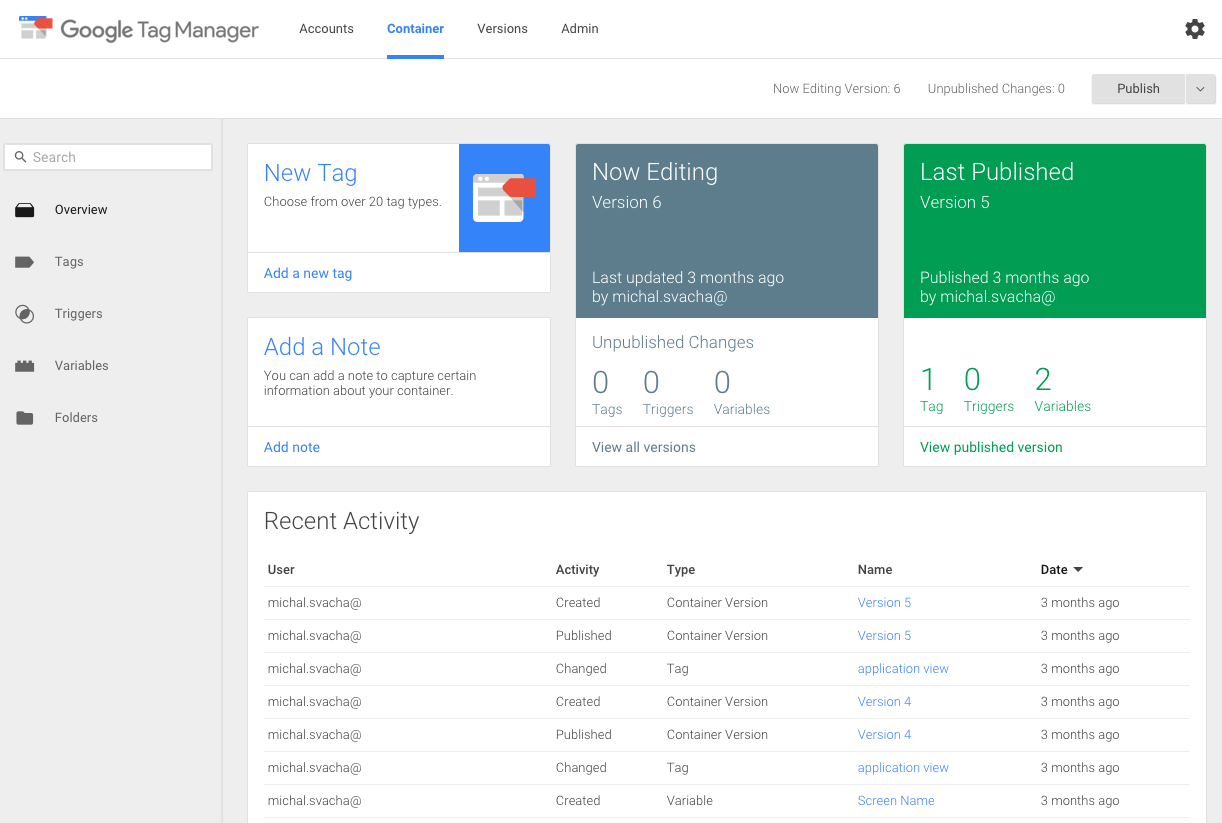
\includegraphics[width=0.65\textwidth]{figures/tagmanager}
    \caption{Google Tag Manager Dashboard}
\end{figure}

The dashboard is similar in style to the Google Analytics one. Tags can be created, modified and linked with a specific Google Analytics query. The same as for Google Analytics holds for Google Tag Manager - everything is closed source and runs exclusively on Google's servers.

\subsection{Tealium}

Tealium is a complex tool combining all marketing tools on the market (Criteo, Socialbakers, but also Google AdWords etc.). It does offer insights into usage and performance and it is very robust. 

\bigbreak

"Combining the leading enterprise tag management solution, an omnichannel customer segmentation and action engine, and a suite of rich data services, the Tealium CDP enables organizations to unlock customer data trapped in siloed marketing systems, build a unified customer view, and take real-time action." \cite{tealium}

\bigbreak

As of December 2015, Tealium successfully completed a Health Insurance Portability and Accountability Act (HIPAA) and Health Information Technology for Economic and Clinical Health Act (HITECH) attestation examination \cite{hipaa}, making it compliant to store data in the cloud securely. The only limitation with this is, that it is only valid in the USA - it does not extend to countries such as China, Japan or Russia, where customer data have to be stored within the country's borders.

The tool itself is intended to be wired up and used as-is. Tealium has their own servers, their won front-end and no API. While for smaller to mid-sized companies it may be sufficient, larger companies require code customizations and integrations into their systems that are currently not provided by this tool.

\subsection{Fabric (formerly Crashlytics)}

Fabric is a platform made by Twitter. Collected and fine-tuned I should say, as it comprises of multiple acquired start-up platforms. The focal point of this platform is a former crash reporting tool Crashlytics \cite{crashlytics}. Aside from that Fabric is a full-featured developer platform used for a variety of tasks. It helps to overcome obstacles a developer may face - even the distribution of beta versions to testers, which has always been a problem for iOS developers.

\bigbreak

"The Fabric platform is made of three modular kits that address some of the most common and pervasive challenges that all app developers face: stability, distribution, revenue and identity. It combines the services of Crashlytics, MoPub,Twitter and others to help build more stable apps, generate revenue through the world’s largest mobile ad exchange and enable to tap into Twitter’s sign-in systems and rich streams of real-time content for greater distribution and simpler identity. Installation takes minutes, and most features only require a few lines of code." \cite{fabric}

\bigbreak

Fabric has been taken it a step further and is not only about reporting crashes, but it also reports overall statistics, like Google. One really nice feature is a video visualization of user movements in the application. Formerly Appsee \cite{appsee}, now a UX part of Fabric, creates a video of steps users take in the application to give the developer a new perspective on how their application is actually used.

The source code of Fabric is closed source (except for some parts, like Fastlane \cite{fastlane}) and all of the statistics run on Twitter's servers. The Data is not accessible in any other way, than via Fabric's custom dashboards. 

The whole platform is free to use. Registration of developers and applications is required along with the installation of a custom Fabric installation program which integrates the framework into existing projects.

\subsection{App Pulse (formerly Pronq)}

Hewlett-Packard Enterprise AppPulse Mobile is a mobile app performance monitoring tool that tracks the real user experience of mobile applications.

App Pulse is very different from the previously listed tools in a way that it reports everything at all times. The usage is fairly low - tens of kilobytes per week, but it is very thorough. Screen time, actions, movements - it is all there in the report and no setup is required for the start. That obviously leads to gathering a lot of junk by default.

Contrary to iOS standards, App Pulse's SDK is distributed via a compiled library that has to be drag-and-dropped manually into the Xcode project. This is not a good practice, as Apple's updates are regular and oftentimes break a lot of old code, so keeping the SDK up to date manually is a lot of pain.

Because it works out-of-the-box and "automagically" tracks everything that happen in the application, the one big issue is the need to have a consistent naming of all views, labels, buttons etc. - as it does everything on its own, without hooking up the actionable items to the framework manually, it can be hard to determine which button was referred to in the report. One really interesting feature is battery level monitoring, though it is disputable, as the user may have multiple applications running in the background.

Free 30-day trial allows up to two mobile applications, 25.000 active users per application (everything above is discarded, or offered for the standard monthly price) and access to the App Pulse community. The tools are closed source and all of the statistics runs on Hewlett-Packard Enterprise servers as it is a Software as a Service (= SaaS). No API is provided.

\subsection{Apteligent (previously Crittercism)}

Apteligent doesn't stand out from previously mentioned tools - it runs on Apteligent's own servers, has custom SDK and works seemlessly. While it does have some benchmarking that others don't, at the end of the day, Apteligent again is the owner of your users' data. It seems very enterprise oriented - it enables 3rd party API integration into their system, which enables monitoring the performance of other APIs used in the application to really find what can be the bottleneck of the overall performance.

The tools are closed source and all of the statistics run on Apteligent's servers. API for data retrieval is provided.

\subsection{New Relic}

Other than the standard package (SDK, custom servers, periodical reports), New Relic has a nice alerting system - when a crash occurs, a web hook to ticketing system can be defined to streamline bug reports into the issue tracker.

Similar to Tealium, New Relic does stand out with the focus on data encryption:

\bigbreak

"You have complete control over what, if any, sensitive information is sent to New Relic. We are unique among software analytics solutions. When you deploy our agent, by default, our security settings and regulatory compliance exceed industry standards, and all data is encrypted in transit." \cite{newrelic}

\bigbreak

While this is a good start, it simply isn't compliant with the legislation of many countries, to store the users' data on a "random" cloud computer storage. The iOS SDK is distributed in a compiled binary file, having enormous 28,5MB. It is not open sourced. API for data retrieval is provided.

\subsection{Apple}

The last tool I will mention isn't considered as a framework, but is important nonetheless. As companies fight for user data from mobile applications - such as Twitter, who even gives out their platform to everybody for free, naturally the platform owners (Apple and Google) strive for keeping all that precious data for themselves. Apple announced in 2015 at their Wordwide Developer Conference (= WWDC) a new iTunes Connect portal with a new feature - App Analytics. 

\newpage

\begin{figure}[!ht]
	\centering
	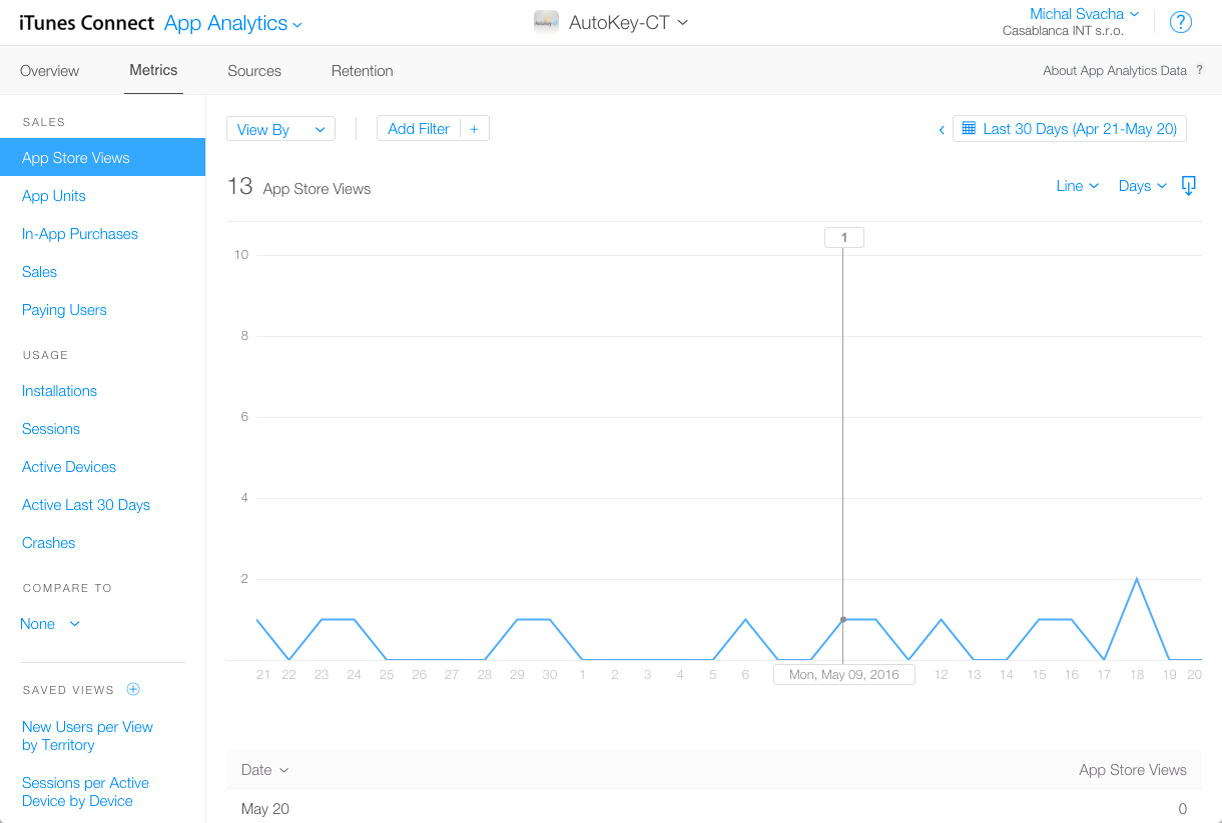
\includegraphics[width=0.65\textwidth]{figures/appleanalytics}
    \caption{Apple App Analytics Dashboard}
\end{figure}

It is fairly thorough in means of usage, downloads, screen time etc., but the overall reporting seems very marketing oriented. Crashes do get reported, but not they are not very detailed compared to Fabric's Crashlytics tool.

One of the biggest obstacles every iOS developer faces is the fact that since iOS 5 \cite{udid} it is not possible to uniquely identify a device. Therefore it is virtually impossible to connect two user entries of the same user if the user deletes and redownloads the application. The only way it could be identified is through Apple's own analytics solution. However, the help tooltip for Installations says:

\bigbreak

"The total number of app installations and redownloads. Installations doesn't include app updates."

\bigbreak

Which looks like Apple disabled identification of the same device for themselves as well. 

App Analytics in iTunes Connect is provided to every single developer automatically for free on the iTunes Connect website. There is no framework to be implemented, the statistics is gathered whether the developer likes it or not. Naturally Apple keeps all of the user data on their servers. Even though iTunes Connect has a JSON REST API, none of the sales or analytics data endpoints are exposed.

\newpage

\section{Conclusion on tools}

\begin{enumerate}
	\item Google Analytics
		\begin{itemize}
			\item[{\bf PROS:}] robustness, reliability, reputation
			\item[{\bf CONS:}] completely proprietary, very low-level
		\end{itemize}
	\item Google Tag Manager
		\begin{itemize}
			\item[{\bf PROS:}] abstraction above GA, flexibility
			\item[{\bf CONS:}] completely proprietary, hard initial setup
		\end{itemize}
	\item Tealium
		\begin{itemize}
			\item[{\bf PROS:}] versatility, omni-channel connectivity
			\item[{\bf CONS:}] completely proprietary
		\end{itemize}
	\item Fabric
		\begin{itemize}
			\item[{\bf PROS:}] versatility, community support
			\item[{\bf CONS:}] completely proprietary, required Twitter registration, data inaccessibility
		\end{itemize}
	\item App Pulse
		\begin{itemize}
			\item[{\bf PROS:}] automatic initial setup
			\item[{\bf CONS:}] completely proprietary, non-standard SDK distribution, data inaccessibility
		\end{itemize}
	\item Apteligent
		\begin{itemize}
			\item[{\bf PROS:}] 3rd party tool integration
			\item[{\bf CONS:}] completely proprietary
		\end{itemize}
	\item New Relic
		\begin{itemize}
			\item[{\bf PROS:}] user data encryption
			\item[{\bf CONS:}] completely proprietary, non-standard SDK distribution
		\end{itemize}
	\item Apple
		\begin{itemize}
			\item[{\bf PROS:}] no installation or setup required
			\item[{\bf CONS:}] completely proprietary, data inaccessibility
		\end{itemize}
\end{enumerate}

None of the tools meet the requirements for deployment (custom servers) and therefore privacy as well for a global enterprise in regulated market. It is necessary to design an architecture that would fit the needs - run the whole solution on custom servers and enable the mash-up of various knowledge resources deployed across the company.

\chapter{Design}

\section{System Architecture}

\begin{figure}[!ht]
	\centering
	\includegraphics[width=0.8\textwidth]{figures/03_design/design_diagram}
    \caption{Proposed Workflow}
\end{figure}

\subsubsection*{Description}

The workflow should be as linear as possible mirroring the natural flow of data. The central knowledge base is the issue tracker, because that's where the project management team defines the objectives set by the top management. The UX team specifically needs to measure certain tasks in the application so it is absolutely valid that they would add their needs to the issue tracker.

From then on, the domain vocabulary is created and stored for everybody to see. In order to measure the tasks performed by the developer (for example "implement login form") using the same domain vocabulary, something has to deliver a computer-readable version of the vocabulary. That is the task of the Semantic Data Manager - to extract the knowledge from the Issue Tracker and serve it to the developer so he/she can use it easily within the application.

The user data is then reported to the Tracking Engine using the same domain vocabulary that was defined at the beginning. That will enable alignment and easy reporting of the results.

\section{Issue Tracker}

Issue Tracker is a software deployed in a company for managing and tracking the work done by multiple employees across different departments. It allows the project management team to define projects and milestones, and to break the work down into tasks and sub-tasks. Those are then assigned to specific people and marked as complete when they're done and reviewed. It is considered good practice for a task/issue to become immutable with respect to its name (and of course project label and ID) when it is created and assigned. A detailed description and comments can be added, but in order to preserve some stability, the name should remain the same.

There are many solutions on the market, such as Bugzilla, JIRA or open-source Redmine. Most of the solutions provide a REST API for third-party integration.

\subsection{Knowledge Structure}

Every company uses a slightly different way of structuring their knowledge in their project management tools. In my situation, the structure is as follows:

\begin{itemize}
	\item Teams
	\item Project
	\item Issues
\end{itemize}

Different tools have different naming conventions, but this structure is as general as possible so it is applicable to most of the tools on the market.

\subsubsection{Teams}

Everybody is distributed into teams in various departments. While departments are important in the company structure, in project management, teams are more relevant. Every team has its own Project Board (either Scrum or Kanban), which reflects the state of the team at the time - how much work has been done, what will be done and what's currently being done.

\subsubsection{Projects}

Each team works on their own projects. Often-times, collaboration does occur, but the owner of the project is still the team. If another person collaborates with another team, it is reflected in his/her work statistics (storypoints, hours spent), but the ownership stays within the scope of the project and thus withing the team as well.

\subsubsection{Issues}

An issue is the most granular entity in the system. It defines a step or set of steps to be performed and is usually assigned to one person. Workflows for reviewing etc. vary from team to team. It is possible to break down the work on a single issue (if it's an especially large one) into sub-tasks, but those are not given IDs, so they are not unique per se. They only serve to increase the clarity and visibility of work being done during the day. When all sub-tasks are finished, the whole issue is finished. That is the state reflected by the API.

\subsection{Knowledge Extraction}

The extraction of the knowledge will build on the premise that some parts of the data at a certain point of time are immutable. In order to make it as bulletproof as possible, I will only assume immutability of the name of the issue, its automatically assigned identifier (ID) and, obviously, the project it belongs to. Everything else is considered fully mutable and is free to be changed in order to provide flexibility.

The idea behind the tracking itself in the same domain vocabulary is that the beginning and end of an issue/task/sub-task are reported, giving a direct feedback on the success or failure of the implemented workflow.

\subsubsection*{Example}

An issue is created in the Issue Tracker - "Create form for user registration.". The Issue Tracker automatically assigns an identifier, for example "SA-01". The resulting database table should look like this:

\bigbreak

\begin{table}[!ht]
\begin{center}
\begin{tabular}{|l|l|l|l|}
\hline
\textbf{Issue ID} & \textbf{Name} & \textbf{Type} & \textbf{...} \\
\hline
SA-01 & Form for user registration. & Start & ... \\
\hline
SA-01 & Form for user registration. & Finish & ... \\
\hline
SA-01 & Form for user registration. & Start & ...\\
\hline
SA-01 & Form for user registration. & Finish & ... \\
\hline
SA-01 & Form for user registration. & Start & ...\\
\hline
\end{tabular}
\end{center}
\caption{Example Database Entries}
\label{tab:ex_db}
\end{table}

It is clear what is measured here\footnote{The "..." marks obvious missing columns, such as timestamp, device type, etc.} - the success of a registration of a new user. For each registration that is begun, there is a "Start" entry. For each successfully finished registration, there is a "Finish" entry. No other KPI was defined to be measured, so without storing any junk data, it is easy to calculate the percentage ($2/3$) of users that successfully registered versus the percentage that didn't ($1/3$).

\subsubsection{Domain-specific Language}

In order to track more than just the beginning and the end of the workflow defined in the scope of the issue, it is necessary to give the stakeholders a way to define certain observable events to pay attention to. Usually, every issue has a field specifically for description, which contains some human-readable set of instructions. Why not piggyback on that and give it just enough structure to make it also computer-readable?

Let's imagine we want to measure how many times the user clicks on the help button in the registration form. Then the database table would be extended to:

\bigbreak

\begin{table}[!ht]
\begin{center}
\begin{tabular}{|l|l|l|l|}
\hline
\textbf{Issue ID} & \textbf{Name} & \textbf{Type} & \textbf{...} \\
\hline
SA-01 & Form for user registration. & Start & ... \\
\hline
SA-01 & Form for user registration. & Finish & ... \\
\hline
SA-01 & Help button pressed. & Action & ...\\
\hline
\end{tabular}
\end{center}
\caption{Extended Example Database Entries}
\label{tab:ex_db2}
\end{table}

Another type has appeared in the database table - "Action". This represents some measurable item, linked to the registration form itself, neatly labeled with the relevant Issue ID, easy to find and in the same domain vocabulary as was intended.

\section{Semantic Data Manager}

This is the most crucial component of the whole solution - connecting the Issue Tracker and tracking capabilities. The main task is to obtain actionable items from the Issue Tracker and create computer-readable domain vocabularies for application engineers to include in their source code. The computer-readable format should in the form of a configuration file. Therefore, there must be a framework that parses such a configuration file and offers in-code assistance for implementing the tracking itself. It goes without saying that the usage should be as smooth as possible.

The configurations produced should be persisted for the sake of reproducibility, though storing any metadata (detailed measurement description) should be avoided as it is subject to change (DSL used in the description). Only the unique issue identifier and its name should be persisted, in order to be able to trace back what the configuration file was meant for. Persisting anything else could lead to disconnection between data and that's exactly what I am trying to solve.

Connecting to the Issue Tracker will be handled via its REST API. It should automatically retrieve a list of all projects and their subsequent issues/tasks/sub-tasks that may or may not contain specific metadata regarding fine-grained measurement demands.

The Semantic Data Manager will run as a stand-alone microservice and will provide a REST API for any kind of UI to be implemented on top of it. It can easily be a website, mobile application or integration into a third-party tool.

\section{Tracking Engine}

The Tracking Engine itself is a completely separate component from the Semantic Data Manager. It can easily be any existing solution, such as Google Analytics or Google Tag Manager. It should be a stand-alone service in which data is stored using the domain vocabularies already obtained.

For reasons listed in the previous chapter, mainly in-house data storage, I will also develop this component and deploy it alongside the Semantic Data Manager. This gives me more flexibility in optimizing the storage and provides the company with a custom tailored solution.

\section{Tracked Device SDK}

The SDK has to have two layers:

\begin{enumerate}
	\item An interpreter of the configuration file from the Semantic Data Manager - load the vocabularies and provide them during the development.
	\item An interface for storing the events - should the Tracking Engine change, the only thing that would be necessary in the application code would be to download dependencies for it and implement the interface. This approach ensures that the in-code measuring always remains the same; only the underlying engine changes.
\end{enumerate}

The whole company runs on iOS devices, so I will develop an iOS framework to be used while developing applications. While iOS may seem limited to only iPhones and iPads, the ecosystem actually enables the frameworks to be written for all Apple platforms - iOS, tvOS and Mac OS X.


\chapter{Implementation}

\section{Deployment}
UML diagram a popis komunikace

\section{Semantic Data Manager}
The central part of the project should be robust and reliable. For that reason I chose Java as the main technology. For convenience and standardization of the code-base I opted for Spring Boot framework.

The code is packaged by Maven and deployed as WAR to AWS EB auto-scaled m3.medium instance, running Tomcat 8 server. Database runs on managed Amazon RDS (Relational Database Service), which is fast, secure and scalable deployment of database engine. The size of the instance is recommended for any application running JVM. The configuration is Intel Xeon E5-2670 v2 (Ivy Bridge), 4GB SSD storage and 3.75GB RAM. Any additional memory is handled via S3.

\section{Tracking Engine}

Because the tracking engine was developed after the Semantic Data Manager, I opted to use Java again. I first tried to use play2 framework for educational purposes, but I encountered too many obstacles deploying play2 application so I had to drop it. Main reason was that play2 uses its own application server - Netty Server, which always runs on port 9000. When deploying to AWS EB (via tool Activator that prepares a package similar to WAR file - WAR files are not supported by play2), NGINX that handles HTTP requests searched for application deployed on port 5000. Because Netty does not support compile-time port configuration and NGINX does not support running Activator to set up the port during run-time I had to drop the idea of using play2. I tried to configure NGINX to not look for the application on port 5000, but AWS EB has a very limited configurability in this area. That was the end for play2 and so I used Spring Boot again.

// JSON

The code is deployed in the same fashion as the Semantic Data Manager.

\section{Statistical Front-end}

\subsection{Numerous}
Numerous has two components and uses monolithic git repository to keep everything together. It is designed to be a standalone micro service and can be used outside of the scope of this solution.

\subsubsection{Back-end}
For computational convenience in future development (= data modeling, model training etc.), Python was selected to be the language this component will be written in.

The code is packaged in Docker image and is deployed in two EC2 t2.medium instances - one for the API and one for the database. The main difference between T2 and M3 is the processor computational power - T2 has Dual Core Intel Xeon 3.3GHz with Turbo. Also it is a Burstable Performance Instance, meaning that it is provided with a baseline level of CPU performance with the ability to burst above. T2 instances are for workloads that don't use the full CPU often or consistently, but occassionally need to burst (computing statistical models for example in my case).

\subsubsection{Front-end}
Requirements for mobile client were only for iOS devices. Therefore, as no code portability was required, I opted to go native. For native development, Apple's language Swift is used (as of March 2016, in version 2.2). Swift is a general-purpose, multi-paradigm (both object oriented and functional), compiled programming language. It was first released to support iOS and Mac OS X, now supporting also tvOS (Apple TV 4th generation and newer) and watchOS (Apple Watch). Many more cases of use are coming, because Swift compiler has been open-sourced. It is gaining popularity among non-Apple developers mainly due to its safety, robustness and ease of use.

\subsubsection*{User Interface}

DASHBOARD screenshot + DETAIL screenshot

Color scheme of the application was provided by a graphical designer. Most of the graphics is set on code level. I am not in favor of bloated projects because of multitude of png files for every possible device. Code generated graphics may introduce some level of complexity, but the space saved on user's device is more important. Even with app-slicing (method of distribution provided by Apple - only the resources needed for your device are downloaded), the amount of space saved is at least 3MB.

ios-charts

\subsubsection*{Networking}

Alamofire + VPN

\subsubsection*{Data Model}

Realm.IO

\subsubsection*{In-app Analytics}

Google Tag Manager

\chapter{Testing}

\begin{itemize}
 \item Způsob, průběh a výsledky testování.
 \item Srovnání s existujícími řešeními, pokud jsou známy.
\end{itemize} 

\chapter{Conclusion}

The aim of this work was to identify disconnected data endpoints and figure out a way how to connect them and make use of them. I demonstrated the need on misunderstandings between different teams and pointed out where value could be more driven.

In the second part, I analyzed the existing tools on the market and I assessed their usability in the given context. Not being fully satisfied with their functions, I took the initiative and designed a system that would be in-house, deployed in the AWS VPC environment. 

In the third and fourth part, I designed and developed the system into a fully viable product (= MVP). As I went along, I kept validating my ideas with my peers and supervisors.

In the last part, I set myself a goal to test the system from many aspects - idea, usabilty and performance. While some tests went better than the others, it brought me so many valuable insights and pointed out places with room for improvement that I hadn't even considered before. For that I see the tests as an immense success, regardless of the actual results - it shows that the idea is valid, people are interested in it and there is something to continue working on.

\section{Technical debt}

Naturally, when a project delivery is time-boxed, certain functions/features get a higher priority than others along the way. This project has been no exception.

\subsection{Semantic Data Manager}

\begin{enumerate}
	\item SSL certificate is only self-signed.
	\item JIRA communication could be abstracted out into another layer to make sure when REST API changes that the rewrites would only happen in the parser.
	\item There is no mechanism for versioning of the configurations.
\end{enumerate}

\subsection{Administration Application}

\begin{enumerate}
	\item Several UI elements need more fine-grained graphics to improve the usability.
	\item There should be a search bar in the issues.
	\item Dropbox integration is only one out of many other possibilities - Syncplicity, E-mail etc. should be supported as well.
\end{enumerate}

\subsection{Tracking Engine}

\begin{enumerate}
	\item SSL certificate is only self-signed.
	\item There is no authentication method for the applications sending data.
	\item The analysis of the data development is currently limited to time series.
\end{enumerate}

\subsection{Timeseries Application}

\begin{enumerate}
	\item There is no user management built in the application.
	\item KPIs can't be added per KPI, only per application.
	\item There is no graph mash-up, only number analysis per day.
\end{enumerate}

\section{Future development}

There is absolutely no shortage of work that can be done on the project. The project is healthy and stable and there are plenty of features that can be implemented in order to drive this project even further. I am very optimistic thanks to the support of all the people that got interested in the project. 

One step at a time, the best thing to do is to take a look and revisit the foundations of the project - the Semantic Data Manager and the Tracking Engine. When these two components are without any technical debt and robust, only the sky is the limit.

%*****************************************************************************

\bibliographystyle{abbrv}
%bibliographystyle{plain}
%\bibliographystyle{psc}
{
\def\CS{$\cal C\kern-0.1667em\lower.5ex\hbox{$\cal S$}\kern-0.075em $}
\bibliography{reference}
}

%*****************************************************************************
\appendix

\chapter{List of abbreviations}

\begin{description}
	\item[AWS] Amazon Web Services
	\item[EB] Elastic Beanstalk
	\item[EC2] Elastic Compute Cloud
	\item[KPI] Key Performance Indicator
	\item[MVP] Minimum Viable Product
	\item[PoC] Proof of Concept
	\item[S3] Simple Storage Service
	\item[SDLC] Software Development Life Cycle
\end{description}
	
\chapter{Instalační a uživatelská příručka}
\textbf{\large Tato příloha velmi žádoucí zejména u softwarových implementačních prací.}
\chapter{Contents of CD}

\begin{forest}
  for tree={
    font=\ttfamily,
    grow'=0,
    child anchor=west,
    parent anchor=south,
    anchor=west,
    calign=first,
    edge path={
      \noexpand\path [draw, \forestoption{edge}]
      (!u.south west) +(7.5pt,0) |- node[fill,inner sep=1.25pt] {} (.child anchor)\forestoption{edge label};
    },
    before typesetting nodes={
      if n=1
        {insert before={[,phantom]}}
        {}
    },
    fit=band,
    before computing xy={l=15pt},
  }
[/
	[src/
    		[java\char`_semantic\char`_data\char`_manager/]
    		[java\char`_tracking\char`_engine/]
    		[swift\char`_administration\char`_app/]
    		[swift\char`_timeseries\char`_app/]
    		[swift\char`_tracking\char`_sdk/]
    		[README.txt]
  	]
  	[text/
  		[src/]
    		[svachmic\char`_thesis.pdf]
  	]
]
\end{forest}



%*****************************************************************************

\end{document}
